
Interesting scattering processes nearly always include charged
particles in the final state. The two tracking systems in ATLAS, the ID and the muon
system, are designed to measure the trajectories of these charged
particles, from which momentum 4-vectors are derived. A track is fully
specified by five parameters $\vect{\alpha} =
(q/p,\theta,\phi,d_0,z_0)$, where $q$ is the charge, $p$ is momentum,
$\theta$ is the angle with respect to the beam line, $\phi$ is the
azimuthal angle, $d_0$ is the distance of closest approach (usually to
the vertex associated to the track) in the
transverse plane, and $z_0$ is the distance of closest approach in the
longitudinal direction. In the following section,
the algorithms for fitting these parameters from detector hits will be
described. 

\subsection{Inside-out Tracks}

The primary tracking algorithm in ATLAS builds tracks starting with
hits in the pixel detectors, and progressively adding hits at larger
$r$ values. This is known as the inside-out track reconstruction
paradigm~\cite{bib:Cornelissen:2007vba}. Starting with hits from the pixel and SCT detectors,
collectively known as the silicon detectors, clusters of contiguous
hits are identified and associated with a coordinate in space. The
track-finding algorithm is seeded by a group of three clusters in
different layers that is consistent with a track. This seed defines a
``road'' along which the track candidate is built. The track
trajectory is propagated through the detector in a Kalman filter based
approach~\cite{bib:Fruhwirth:1987fm}. At the $k^{\textrm{th}}$ detector layer, the hit
that is most consistent with the track parameters from the previous
layer is assigned to the track. The track parameter vector is then
updated with the new hit included, yielding $\vect{\alpha}_k$. The propagation to the subsequent
layer is then given by

\begin{equation}
\vect{\alpha}_{k+1} = M_k\vect{\alpha}_{k} + \vect{\epsilon}_{k}
\end{equation}

\noindent
where $M_k$ is the linear map representing the magnetic field between the
two detector layers, and $\epsilon_{k}$ is a stochastic term that
accounts for multiple scattering of the charged particle. The
procedure is then repeated at layer $k+1$. The above approach for
fitting the track parameter vector is equivalent to a global minimum
least-squares fit. 

After all of the seeds have been evaluated by the Kalman-filter
algorithm, ambiguities are removed from the resulting track candidate
collection. These ambiguities include track candidates that share one
or more hits, are incomplete, or include hits that arise from more
than one charged particle. In order to resolve these ambiguities, the
tracks are first refitted using a detector geometry with a more
realistic description of the detector material. Each track is then
assigned a score that quantifies the quality of the track. Tracks with
more hits receive higher scores, and these scores are weighted
according to the precision of the detector subsystem in which the hits
reside. Given the high intrinsic efficiencies of the silicon
detectors, if a hit is absent along a track trajectory, the track
score is penalized. After track scoring, hits that are shared by more
than one track are assigned to the track with higher score. The
remaining track is then refitted and re-scored. Tracks that fail to
pass a score threshold are discarded.

The silicon only track candidates that pass the quality threshold are
the seeds for the extension of the track into the TRT. In
the first pass, the silicon hits that define the track seed for the
TRT extension are not changed. Again, the Kalman filter approach is
used to map the track from one detector surface to another. Along the
trajectory, TRT hits are added depending on the distance between the
Kalman filter prediction and the actual hit location. With the TRT hits
identified, the track is refitted with the hits from all
sub-detectors-- silicon and TRT. In this pass, the silicon hits are
allowed to vary. The score of the refitted track is compared to that of
the silicon only track, and if it is smaller, the silicon only track
is retained, with the hits from the TRT as outliers, but still
associated to the track. If the score of the refitted track is larger,
this new track is retained. 

\subsection{Outside-in Tracks}

Because the inside-out algorithm is seeded by silicon clusters
associated to a primary vertex, it fails to find tracks arising from
secondary decays that occur late in the silicon system or in the
TRT. These tracks include those associated with electrons
from photon conversions or leptons from in-flight hadron
decays. To recover secondary tracks, an outside-in algorithm, starting
in the TRT, is used in concert with the inside-out algorithm. 

Since TRT hits do not have information about the global $z$
coordinate in the barrel, it is not possible to use pattern-finding
procedure based on three-dimensional space coordinates as is done in
inside-out tracking. Instead, the TRT hits are projected to the
$r-\phi$ plane in which they form straight lines. The hits are then Hough
transformed~\cite{bib:Duda:1972uht} to the parameter
space of a line, where the coordinates are the $y$-intercept, or the
initial $\phi$ of the line, and the slope, or $1/p_{\textrm{track}}$,
where $p_{\textrm{track}}$ is the momentum of the track. In this
space, track candidates appear as maxima at their respective
($\phi_0,1/p_{\textrm{track}}$) coordinates. This technique, which
defines the hit $r-\phi$ coordinate to be the center of the straw,
fails to incorporate information about the drift time. In a second
step, the track candidates are refitted with a Kalman-filter-based
algorithm that incorporates information about the drift time, thereby
improving the accuracy of the fitted track parameters. 

The final step of the outside-in track reconstruction algorithm is the
extension of the TRT segments into the silicon tracker (need good
reference for this). Scanning longitudinally in a small $r-\phi$ wedge
defined by the TRT segment, the algorithm searches for at least two
clusters of SCT hits in the three outermost layers of the
SCT. Once found, the curvature defined by these two three-dimensional
points and the first TRT hit in the TRT segment is computed, and if
the result is unreasonable, the two clusters are disregarded. The SCT
clusters that are retained seed the track-fitting algorithm, which
propagates the track to smaller $r$, extracting the fitted track
parameters. 

\subsection{Vertex Reconstruction}

The vertex of a track refers to the three-dimensional spatial
coordinate from which it originates. Primary vertices are associated
with tracks that have likely been produced as a result of $pp$
scattering in the interaction region, while secondary vertices are
associated with tracks that result from in-flight decays of unstable
particles, e.g. \kshort~decays, or from interactions with the detector
material, e.g. photon conversions. Robust reconstruction of primary
vertices is crucial for suppressing backgrounds due to in-time
pileup. Moreover, the identification of $b$-quark initiated jets,
which is needed to reject top quark processes in the VBF analysis,
relies on the ability to detect displaced vertices close to the
interaction region. 

Reconstruction of primary vertices is split into two
steps~\cite{bib:ATLAS-CONF-2010-069,bib:Piacquadio:2008zzb}. The first
is the identification of vertex candidates based on track parameters
from the reconstructed track collection defined in the previous two
sections. In order to isolate tracks that are consistent with primary
vertices, requirements are placed on the track \pt, \dzero,
$\sigma (\dzero)$, $\sigma (\zzero)$, and the number of hits in the silicon
detectors. In this case, \dzero and \zzero are measured with respect to the
center of the luminous region, also known as the beam spot. The
luminous region is determined for each collision run in an unbinned
likelihood fit to the distribution of primary vertices recorded in the
run. Primary vertices in this fit are reconstructed on-the-fly with a
fast reconstruction algorithm, trading off accuracy for
speed~\cite{bib:ATLAS-CONF-2010-027}. With the tracks selected, the
vertex-finding algorithm scans the $z_0$ distribution, and each maximum is
retained as a seed for a vertex candidate. 

The second step in vertex reconstruction is the fitting of the
vertex position and error with the constituent tracks. Starting with
an initial guess of the vertex position, the $\chi^2$ is computed for
each track. Tracks that are incompatible with the vertex position, as
measured by the $\chi^2$, are de-weighted. For the next iteration, the
vertex position is updated by minimizing

\begin{equation}
L(\vect{v}) = \frac{1}{2}\sum_{i=1}^{n} w(\chi_n(\vect{v})) \chi^2_n(\vect{v})
\end{equation}

\noindent
with respect to $\vect{v}$, the vertex position. Here the sum over the
weighted $\chi^2$s is over the tracks associated with the vertex. Tracks that are
incompatible with the fitted vertex by more than $7\sigma$ are used to
seed a new vertex. 

As the amount of pileup in the ATLAS detector increases, the vertex
reconstruction efficiency decreases~\cite{bib:2012jma}. The primary cause of this is that
with high vertex density, two true vertices are more likely to be
reconstructed as a single vertex. This effect can be mitigated by
placing more strict quality requirements on the tracks that define
vertices. In addition to degraded reconstruction efficiency, high
pileup results in a greater likelihood to reconstruct a fake vertex
due to high hit densities in the ID. The amount of in-time pileup is
reflected by the mean number of interaction per bunch crossing,
$\left \langle \mu \right \rangle$, defined as 

\begin{equation}
\left \langle \mu \right \rangle = \frac{L\cdot\sigma_{\textrm{inel}}}{n_{\textrm{bunch}}f_r}
\end{equation}

\noindent
where $L$ is the measured instantaneous luminosity, $\sigma_{\textrm{inel}}$ is
the inelastic cross section of $pp$ scattering, $n_{\textrm{bunch}}$
is the number of proton bunches in the beam, and $f_r$ is the
frequency of revolution in the LHC ring. The dependence of the vertex reconstruction
efficiency and the fake probability on $\left \langle \mu \right \rangle$ is shown in
figures~\ref{chap:reconstruction:fig:vtx_mu}\subref{chap:reconstruction:fig:vtxeff_mu}
and~\subref{chap:reconstruction:fig:vtxfake_mu}. With
$\left \langle \mu \right \rangle=1$, the efficiency of reconstructing a vertex with strict track
requirements is 90\%, decreasing to about 60\% for $\left \langle \mu \right \rangle=41$, a large
dependence on pileup in spite of the robust track cuts. The
probability of reconstructing a fake vertex, on the other hand, is
insensitive to pileup with robust tracks. If the default track
selection is used, the fake probability goes from 0\% at $\left \langle \mu \right \rangle=1$ to
$7\%$ at $\left \langle \mu \right \rangle=41$. In figure~\ref{chap:reconstruction:fig:mu_nvtx},
the number of reconstructed vertices (\nvtx) is plotted as a function
of $\left \langle \mu \right \rangle$ with strict requirements on the vertex tracks for ATLAS data
collected at $\rts=7$~\tev. The relationship between \nvtx and $\left \langle \mu \right \rangle$
is linear at low $\left \langle \mu \right \rangle$, but as pileup increases, since the vertex reconstruction
efficiency decreases, \nvtx falls below the linear extrapolation. 

\begin{figure}[h]
  \centering
  \subfigure[Vertex reconstruction efficiency]{
  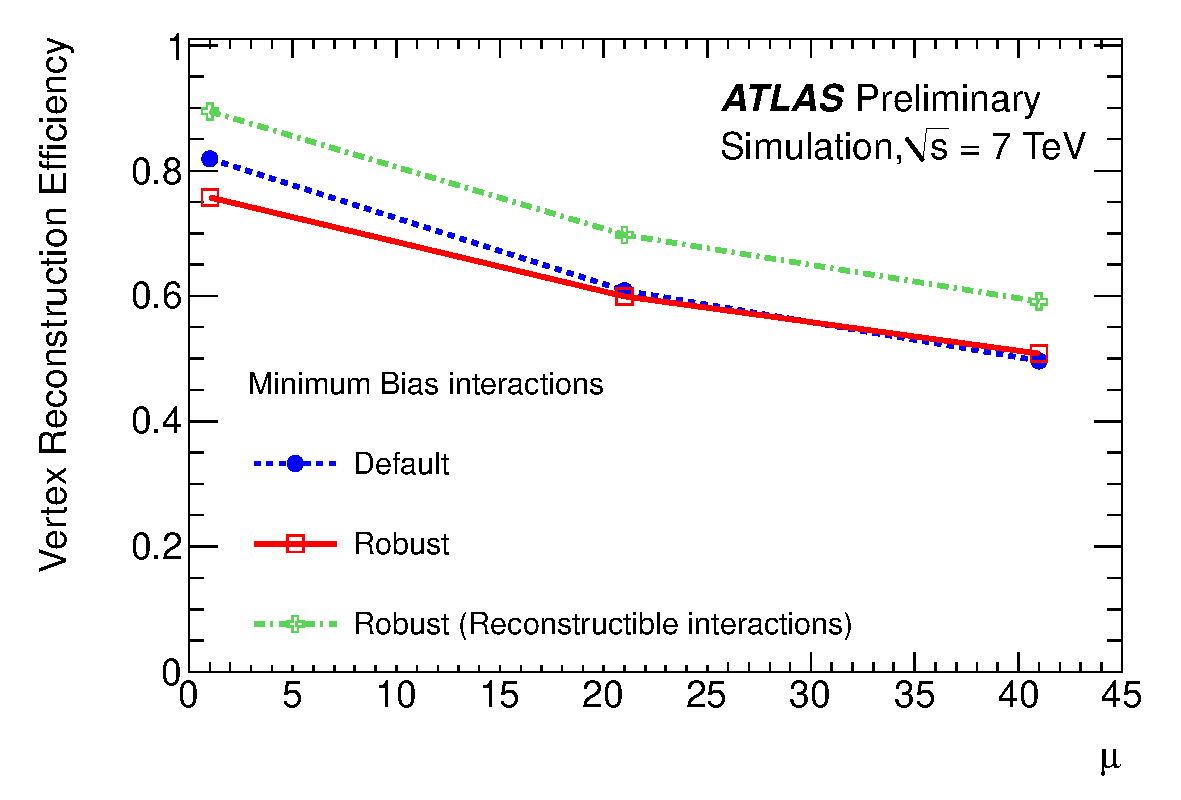
\includegraphics[width=0.45\textwidth]{fig/reconstruction/vtxeff_mu.pdf}
  \label{chap:reconstruction:fig:vtxeff_mu}
  }
  \subfigure[Fake vertex probability]{
  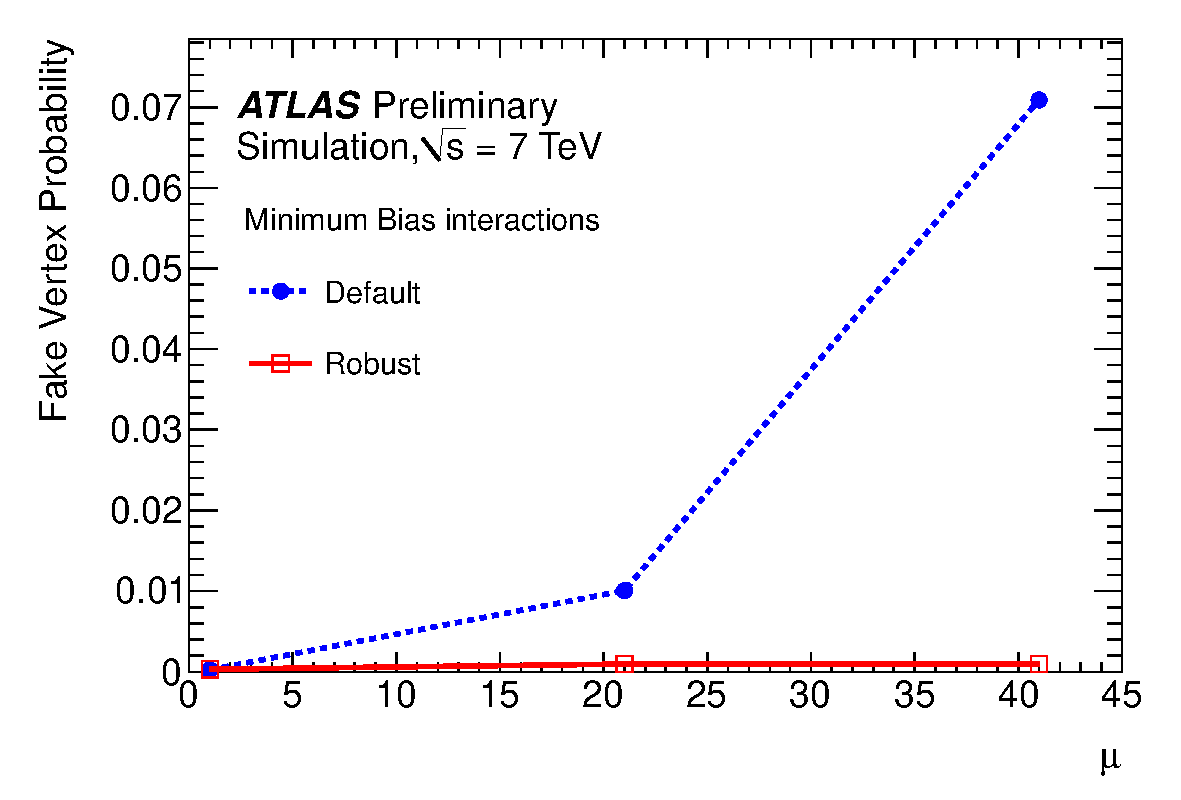
\includegraphics[width=0.45\textwidth]{fig/reconstruction/vtxfake_mu.pdf}
  \label{chap:reconstruction:fig:vtxfake_mu}
  }
  \caption{The vertex reconstruction
  efficiency~\subref{chap:reconstruction:fig:vtxeff_mu} and fake vertex
  probability~\subref{chap:reconstruction:fig:vtxfake_mu} for minimum
  bias MC simulation. Vertices built from default track requirements
  are shown in blue and those built from more strict requirements are
  shown in green and red.\cite{bib:2012jma}}
  \label{chap:reconstruction:fig:vtx_mu}
\end{figure}

\begin{figure}[h]
  \centering
  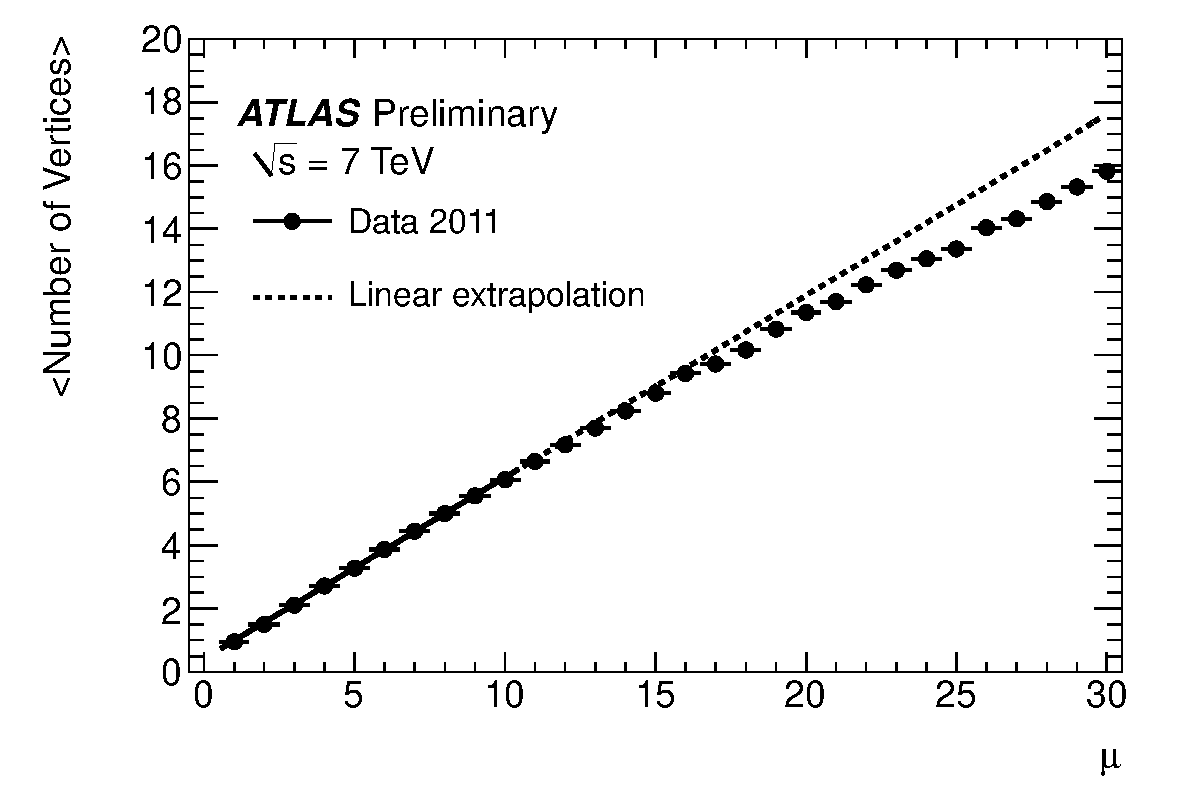
\includegraphics[width=0.6\textwidth]{fig/reconstruction/mu_v_Nvxt.pdf}
   \caption{The number of primary vertices as a function of $\left \langle \mu \right \rangle$ for
  ATLAS data collected at $\rts=7$~\tev.}
  \label{chap:reconstruction:fig:mu_nvtx}
\end{figure}
